\documentclass[a4paper, 11pt]{tufte-handout}
\usepackage[margin=0.8in]{geometry}
\usepackage{framed}
\usepackage{graphicx}
\usepackage{xcolor}
\usepackage{verbatim}
\usepackage{blindtext}
\usepackage{xcolor}
\usepackage{multicol}
\usepackage{mdframed}
\usepackage{amssymb}
\usepackage{indentfirst}
\usepackage{hyperref}
%\usepackage{tufte-book} % or
\usepackage{tufte-handout}% for a handout
% \usepackage{txfonts}
\usepackage{amsmath}
\usepackage{titling}
\usepackage{titlesec}
\usepackage[brazil]{babel}
\definecolor{LightGray}{gray}{0.97}
\usepackage{minted}
\usepackage{xcolor} % to access the named colour LightGray

\setminted[fortran]{  framesep=2mm,
  baselinestretch=1.2,
  bgcolor=LightGray,
  fontsize=\footnotesize,
  linenos}

\setminted[bash]{
  framesep=2mm,
  baselinestretch=1.2,
  bgcolor=LightGray,
  fontsize=\footnotesize,
  linenos=false
}

\titleformat{\section}{\normalfont\Large\bfseries}{\thesection}{1em}{}[\titlerule] 
\titleformat{\subsection}{\normalfont\large\bfseries}{\thesubsection}{1em}{} 
% \renewcommand\thesubsection{\Alph{subsection}}
\graphicspath{ {./graficos/} }

\hypersetup{
  pdfauthor={Jefter Santiago},
  pdftitle={Projeto 3 - Equações de Onda II (Análise de Fourier)},
%  pdfkeywords={},
%  pdfsubject={Anotações métodos matemáticos aplicados à física},
  pdfcreator={Jefter Santiago}, 
  pdflang={Portuguese},
  colorlinks=true,    % Color links instead of boxes
  linkcolor=blue,     % Color of internal links
  citecolor=green,    % Color of citation links
  urlcolor=blue,      % Color of URLs
}

\begin{document}
\noindent
\large\textbf{Autor:} Jefter Santiago \hfill \textbf{Projeto 3: {\color{blue}\emph{Equações de Onda
      II - Análise de Fourier}}}   \\
\#USP: 12559016 \\
\normalsize Curso: Física Estatística Computacional \hfill 2024.1 \\
Prof. F. C. Alcaraz \hfill Data de entrega: 13/04/2024\\
\noindent\rule{7in}{2.8pt}

\section{Introdução}


Partimos das relações estudadas anteriormente, sendo elas a transformada de Fourier discreta (\verb|DFT|)

\begin{equation}
  \mathcal{Y}_k = \sum_{\ell = 0}^{N/2-1} y_\ell e^{2\pi i \left( k\ell/N \right)}
  \label{eq:dft} 
\end{equation}
\begin{equation}

 onde \( N \) é o número de amostradas utilizadas e \( y_\ell \) são resultados gerados pela
 solução da equação de onda do projeto anterior, observada em apenas um ponto do espaço, fixo.

 
\begin{equation}
  \mathcal{Y}(i, n+1) = 2 \left( 1 - r^2 \right) \mathcal{Y}(i, n) + r^2 \left( \mathcal{Y}(i+1,n) + \mathcal{Y}(i-1,n) \right) - \mathcal{Y}(i,n-1)
  \label{eq:ondas_discreta}
\end{equation}

Com esses resultados vamos fazer análise espectral de potências das componentes de Fourier de
amplitudes de onda para um tempo total observado.
  
\begin{equation}
  P(\mathcal{F}) = \mathbb{R}(\mathcal{F})^2 + \mathbb{I} (\mathcal{F})^2
  \label{eq:espectro_potencia}
\end{equation}

onde \( \mathcal{F} \) é referente à frequência das componentes real e imaginária.

Com isso temos as ferramentas que vão ser utilizadas para estudar oscilações em uma corda com
condições de contorno fixas e com uma extremidade solta.


\section{Simulação de ondas em cordas}
\label{sec:borda-presa}
  

Iniciamos o projeto e portanto a discussão com condição de contorno de bordas presas.Podemos
mapear o sistema da corda com bordas presas para uma \emph{EDP}
com condições de contorno \( Y(0, t) = 0 = Y(L, t) \). Por algum método como separação
de variáveis ou utilizando funções \( f(x \pm vt) \) quaisquer\footnote{Que obedecem as condições de contorno.}
podemos estudar o comportamento da onda no espaço. Partindo disso, temos que em
\( x \), a onda pode ser descrita por uma \emph{EDO} da forma \( \mathcal{X}(x) = A \cos (k x) + B \sin
(kx)\). Pelas condições de contorno da $Y(x, t)$ temos que \( \mathcal{X}(0) = 0 \Rightarrow A = 0 \), logo nossa
solução será apenas em termos de senos. Segue que \( \sin (k x ) = 0 = \sin (k L) \Rightarrow k_n = \frac{n \pi
}{L}\), \( n = 1, 2, 3, ...\) é a solução fundamental de \( \mathcal{X} \), ou seja, descreve o comportamento
da onda em relação aos modos normais dela.


Utilizando a relação para os modos normais \( k_n \) podemos obter uma relação para os comprimentos
de onda para cada um deles, pois \( k_n = \frac{2\pi}{\lambda_n} \), então

\begin{equation}
  \lambda_n = \frac{2 L}{n}
  \label{eq:lambdan}
\end{equation}


Partindo da (\ref{eq:lambdan}) podemos obter uma expressão para as frequências para os modos, isto é
\( f_n = c / \lambda_n \)  nos leva à 

\begin{equation}
  f_n = \frac{n c}{2 L}
  \label{eq:freqn}
\end{equation}



Um detalhe importante para as análises que vamos fazer é o impacto das condições iniciais
escolhidas. O perfil inicial, isto é, a posição \( x_0 \) escolhida para fixar a amplitude gaussiana
no inicio da simulação determina a quantidade de modos fundamentais a oscilação vai ter.

Mais que isso, a posição inicial escolhida pode contribuir para formação dos nós já que de acordo
com simétria de onde parte vai gerar interferências destrutivas. Isso também vale para as outras
interferências, dependendo da fase de \( \pi \) entre as ondas propagantes à esquerda e direita
partindo de \( x_0 \) podem haver componentes componentes que ao realizar transformada de
Fourier(\ref{eq:dft}) vão possuir contribuir com maiores amplitudes.



Com isso temos como qual deve ser o comportamento esperado da transformada de Fourier para pontos
obtidos em uma posição de observação \( x \), isto é, a frequência base será \( f_1 = c / 2L \) onde
\( c = 300  \) (m/s) e \( L = 1  \) (m), então \( f_1 = 150  \) (Hz) escrevemos a frequência
fundamental desse caso como

\begin{equation}
  f_n = n f_1
  \label{eq:freq_fund}
\end{equation}


Tratar o caso de uma borda solta, as relações para comprimento de onda e frequência passam a ser


\begin{equation}
  \lambda_n =  \frac{2L}{n - \frac{1}{2}}
  \label{eq:freq-fund-solta}
\end{equation}


\begin{equation}
  f_n = \left( n - \frac{1}{2} \right) \frac{c}{2L}
\end{equation}


Consequentemente a frequência fundamental \( f_1 \) nesse caso passa a ser \( f_1 = \frac{c}{4L} =
75 \) (Hz) e as próximas são

\begin{equation}
  f_n = \left( 2n - 1 \right)f_1
\end{equation}



\subsection{Implementação}
Segue abaixo as rotinas utilizadas para simulações do projeto.
Primeiramente temos a rotina \verb|DFT(Y, N, DT)|, relativa ao primeiro projeto e apenas com
modificação para armazenar o espectro de potências (\ref{eq:espectro_potencia}):


\begin{minted}{fortran}
      subroutine dft(Y, N, dt)
      implicit real*8 (a-h,o-y)
      implicit complex*8(z-z)

      parameter(pi = acos(-1.0e0))
      dimension Y(4000)

      zi = (0.0, 1.0)
      open(unit = 2, file = "saidas/dft-item-a.dat")
      zeta = exp(2.d0*pi*zi/N)

      do k = 0, N/2 - 1
         zY = 0
         do m = 2, N 
            zY = zY + Y(m)*zeta**(k*m)
         end do

         res =  real(zY)**2 + aimag(zY)**2
!         res = res / (N/2)
         freq = k/(N*dt) 
         print *, freq, res
         write(2, '(3000F20.8)') freq, res
      end do
      close(2)
      end subroutine dft
\end{minted}

Os resultados da execução são armazenados no diretório \verb|saidas/|.

Abaixo está o código das subrotinas referente ao projeto anterior, propagação de ondas em uma corda
fixa, livre e uma rotina para escrever evolução temporal do perfil da onda \verb|DRIVE_WAVE_FIXED(GRID, NX, R)|,
\verb|DRIVE_WAVE_FREE(GRID, NX, R)|,\verb|SAVE_WAVE_STATE(GRID, NX)|, respectivamente.



\begin{minted}{fortran}  
      subroutine drive_wave_fixed(grid, nx, r)
      implicit real*8(a-h, o-y)
      dimension grid(1000, 3)
!     y_next = 2(1-r^2)y_curr + r^2[y(t+1,n)+y(t-1,n)] - y_prev
      grid(1, 3) = grid(1, 2)
      grid(nx,3) = grid(nx, 2)
      y = 2.e0*(1.e0-r*r)
      do i = 2, nx-1
         grid(i,3)=y*grid(i,2)+r*r*(grid(i+1,2)+grid(i-1,2))-grid(i,1)
      end do
      grid(:, 1) = grid(:, 2)
      grid(:, 2) = grid(:, 3)
      end subroutine drive_wave_fixed

      subroutine drive_wave_free(grid, nx, r)
      implicit real*8(a-h, o-y)
      dimension grid(1000, 3)
!     y_next = 2(1-r^2)y_curr + r^2[y(t+1,n)+y(t-1,n)] - y_prev
      grid(1, 3) = grid(1, 2)

      y = 2.e0*(1.e0-r*r)
      do i = 2, nx-1
         grid(i,3)=y*grid(i,2)+r*r*(grid(i+1,2)+grid(i-1,2))-grid(i,1)
      end do

      grid(nx, 3) = grid(nx-1, 3)
      grid(:, 1) = grid(:, 2)
      grid(:, 2) = grid(:, 3)

      end subroutine drive_wave_free
 

      subroutine save_wave_state(grid, nx)
      implicit real*8(a-h, o-y)
      dimension grid(1000, 3)
      write(1, '(3000F16.8)') (grid(i, 2), i=1, nx)
      end subroutine save_wave_state

\end{minted}




Por último temos a função utilizada para escrever os perfis iniciais de onda em forma de pacotes
gaussianos dada por \verb|GAUSSIAN(X, X0, SIGMA)|:
\begin{minted}{fortran}
  function gaussian(x, x0, sigma)
  implicit real*8(a-h, o-y)
  gaussian = exp(-((x-x0)**2)/(sigma)**2)
  end function gaussian
\end{minted}


Partindo dessas rotinas e função podemos montar a simulação completa, presente no arquivo
\verb|tarefa-1-12559016.f|

\begin{minted}{fortran}

      implicit real*8(a-h,o-y)
      implicit real*8(l-l)
      implicit complex*8(z-z)

      external gaussian

      dimension grid(1000, 3)
      dimension Y(4000)

      nx = 1000
      nt = 4000
      r = 1.0d0
      L = 2.0d0
      c = 300.0d0
      dx = L / (nx*1.d0)
      dt = r * dx / c

      print *, "Paramêtros:"
      print *, "----------------------"
      print *, "r = ", r
      print *, " nx = ", nx
      print *, " nt = ", nt
      print *, " L = ", L
      print *, " t = ", nt * dt
      print *, " dx = ", dx
      print *, " dt = ", dt
      print *, "----------------------"

!     aplica as condicoes iniciais ao grid
!     t = 0
      print *, "x0 = ", L/2.0d0
      print *, "σ = ", L/30.0d0

      open(unit = 1, file = "saidas/evolucao-item-a.dat")

      do i = 1, nx 
         grid(i, 2) = gaussian(i*dx, L/2.0d0, L/30.d0)
      end do

      grid(:, 1) = grid(:, 2)
      grid(:, 3) = 0.d0
      call save_wave_state(grid, nx)

!     posicao x = L/4 no vetor das ondas.
      ni = nx / 4 
      print *, "Posicao L/4 = ", ni
      
      Y(1) = grid(ni, 2)

      do i = 3, nt
         call drive_wave_fixed(grid, nx, r)
!         call drive_wave_free(grid, nx, r)
         call save_wave_state(grid, nx)
         Y(i) = grid(ni,2)
      end do
      close(1)

      call dft(Y, nt, dt)
      end
\end{minted}


Nesse arquivo principal foram feitas todas as simulações do projeto. Dessa forma, para executar
rotina de ondas com bordas fixas ou solta basta comentar ou descomentar a linha relativa à chamada
dessas rotinas.

Como foi dito, todas as rotinas estão espalhadas pelo diretório central, sendo os arquivos delas

\verb|rotinas-ondas-12559016.f| e \verb|rotinas-dft-12559016.f|. Além desses arquivos também há um
arquivo tipo \verb|Makefile| que compila essas rotinas. Não há nada de especial nele, apenas
automatização do comando

\begin{minted}{bash}
  gfortran tarefa-1-12559016.f rotinas-ondas-12559016.f rotinas-dft-12559016.f -o   tarefa-1-12559016.exe
\end{minted}

Em todas as simulações os paramêtros utilizados foram mantidos fixos com \( \sigma = L/30 \) e a posição
de observação sendo em \( x = L/4 \). Foi estudado a propagação de onda e
feita análise do espectro de potências para diversos casos de posições iniciais \( x_0 \) para pulso do perfil
gaussiano.


\clearpage
\subsection{Simulação para \( x_0 = L/2 \) }

Como podemos ver a simulação está centrada na origem e ocorrem as reflexões em \( x = 0 \) e \( x = L \).

\begin{figure}[h!] 
    \centering
    \caption{}
    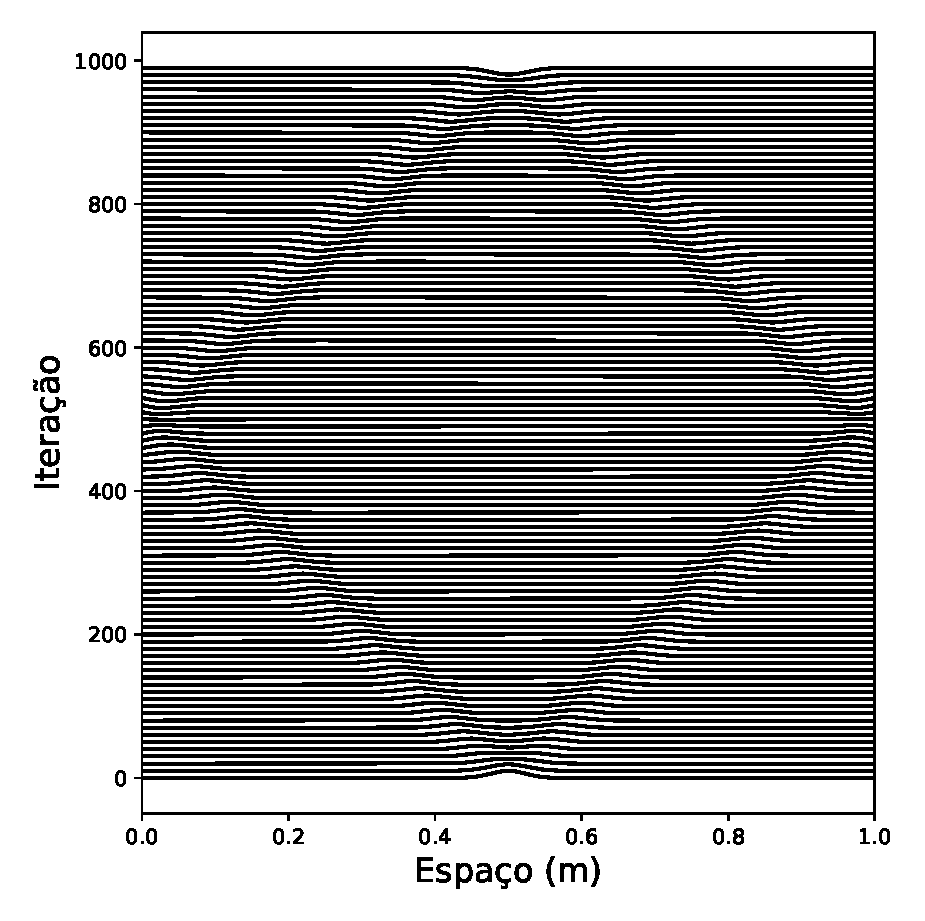
\includegraphics[width=0.45\textwidth]{evolucao-item-a}
    \label{fig:evolucao-item-a}
\end{figure}


Com isso temos o resultado para o espectro de potências sendo (\ref{fig:dft-item-a}). A simetria da escolha de \( x_0 \) 
implica em apenas modos impáres contribuirem para perfil da oscilação.

\begin{figure}[h!] 
    \centering
    \caption{}
    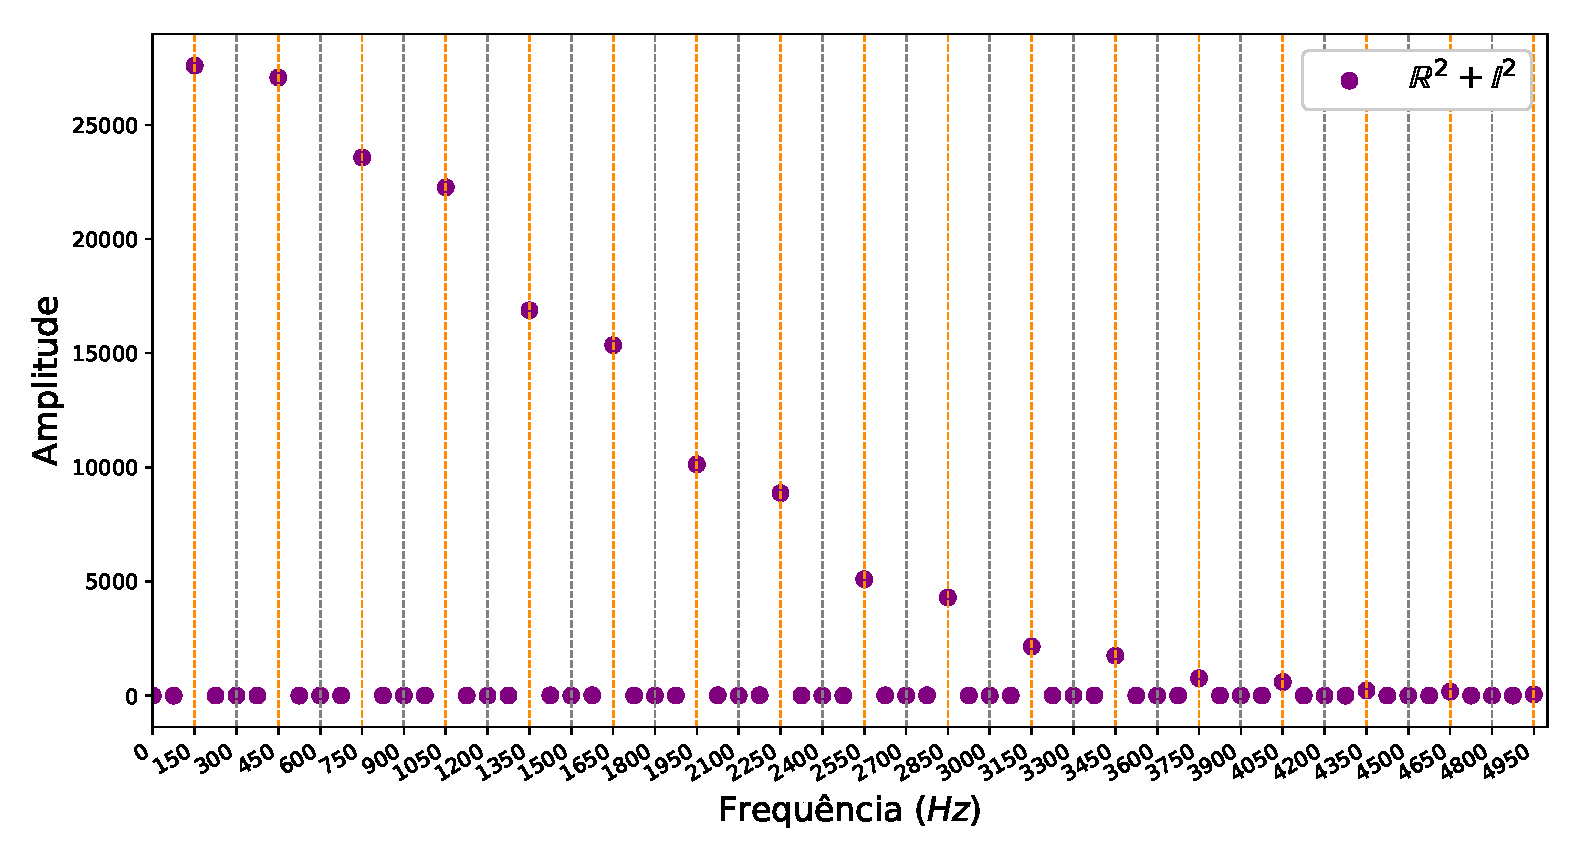
\includegraphics[width=0.65\textwidth]{dft-item-a}
    \label{fig:dft-item-a}
\end{figure}

Nota-se que, como foi dito na discussão em (\ref{sec:borda-presa}) surgem modos fundamentais
de frequência igual à \( f_n = n \cdot 150 \)  (Hz) e esse é o resultado que foi obtido no projeto
anterior para esses paramêtro, já que \( \lambda = 2  \) (m). Além disso, podemos ver na 
(\ref{fig:dft-item-a}) que os tracejados em cinza são referentes à frequências multiplas de \( 300
\) (Hz) que não fazem parte do conjuto de modos fundamentais.


\clearpage
\subsection{Simulação para \( x_0 = L/4 \) }

A posição \( x_0 \) coincide com a posição em que fazemos nossa observação. Como foi discutido em
(\ref{sec:borda-presa}), não será possível observar os modos múltiplos $4$, é como ter posicionado o
``sensor'' em um dos modos e amplitude é fixa igual à zero.

\begin{figure}[h!] 
    \centering
    \caption{}
    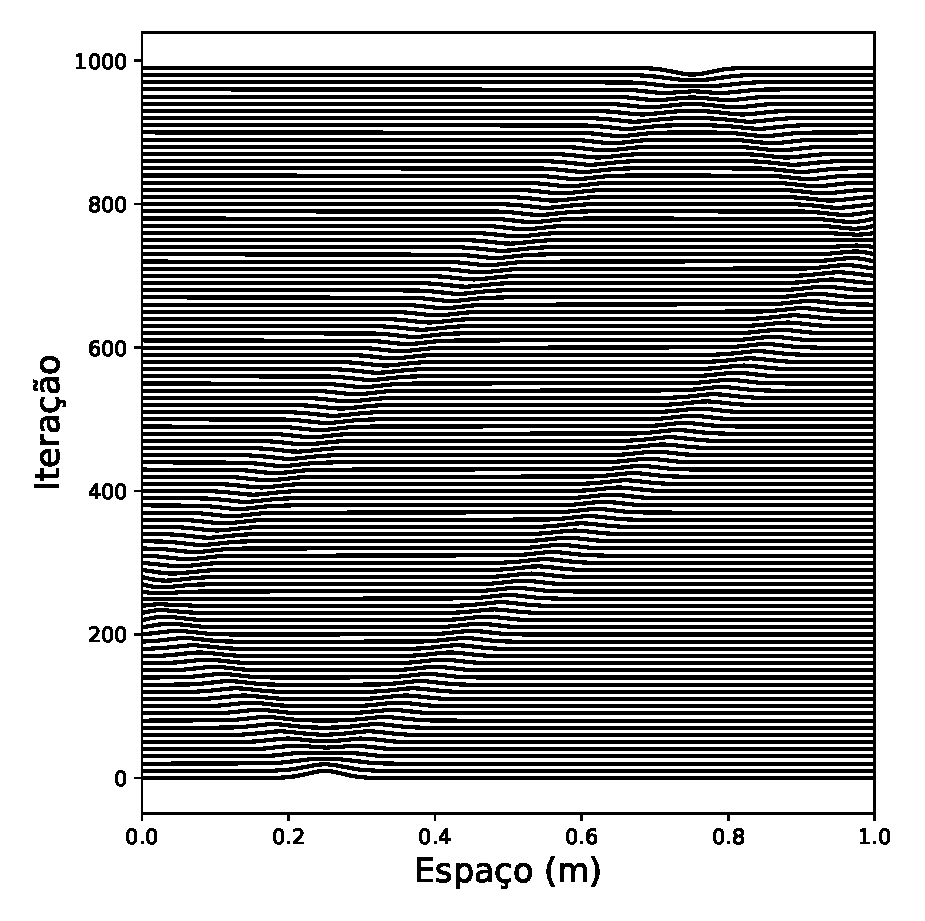
\includegraphics[width=0.45\textwidth]{evolucao-item-b}
    \label{fig:evolucao-item-b}
\end{figure}


Pelo gráfico (\ref{fig:dft-item-b}) podemos ver que de fato frequências múltiplas de \( 4 f_1 \) não
fazem parte do espectro.


Além disso as frequências pares que compoõe o espectro tem amplitude maiores que às impares. 


\begin{figure}[h!] 
    \centering
    \caption{}
    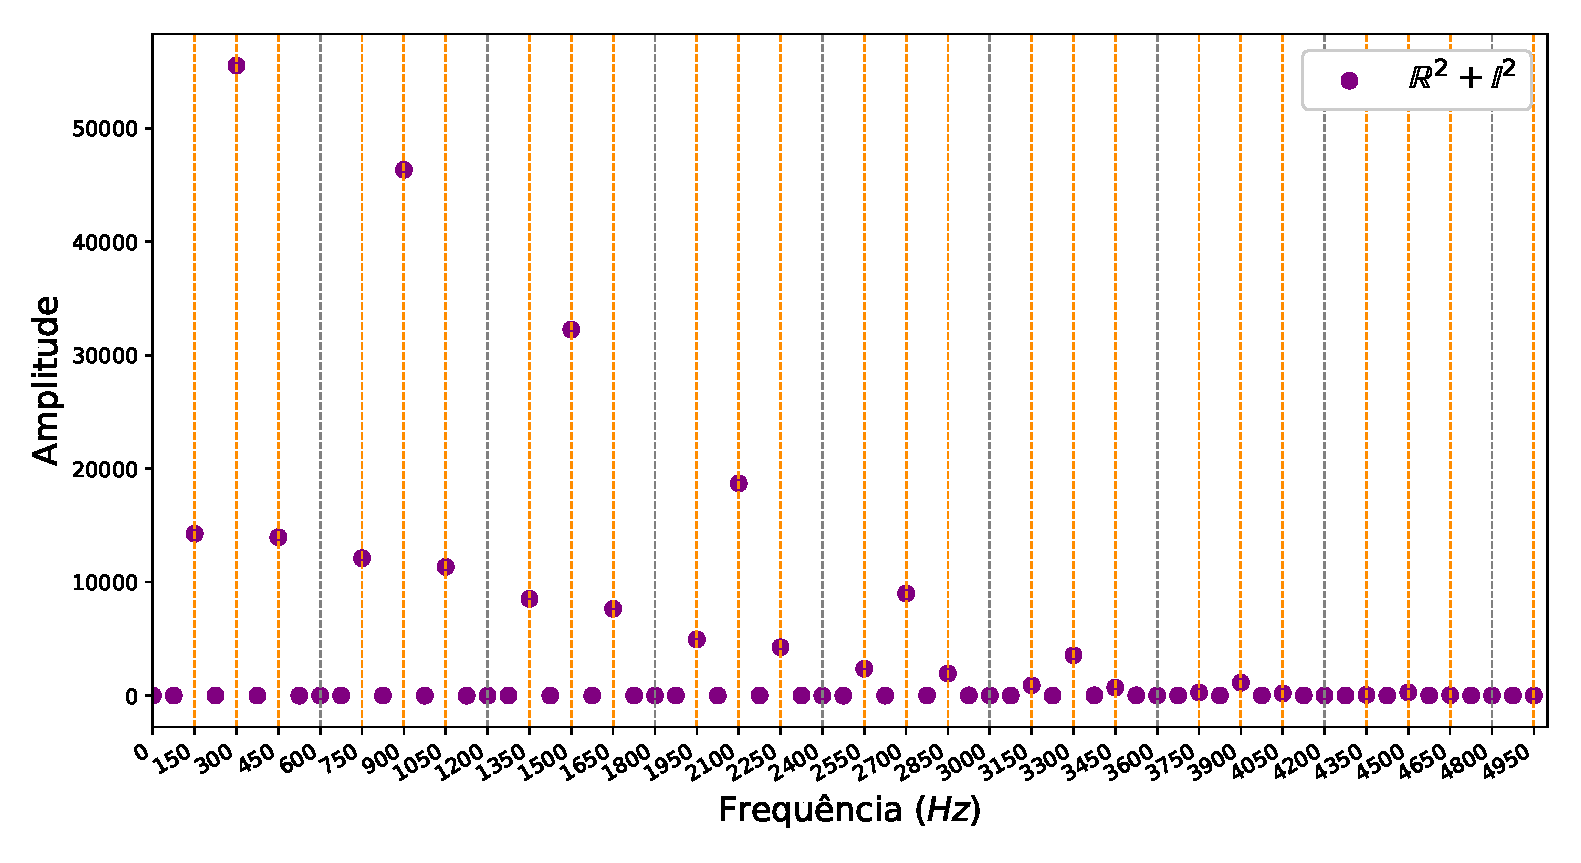
\includegraphics[width=0.65\textwidth]{dft-item-b}
    \label{fig:dft-item-b}
\end{figure}

\clearpage
\subsection{Simulação para \( x_0 = L/3 \) }

Mais uma vez os modos referentes à parte das frequências fundamentais não estão presente nas
componentes espectrais em (\ref{fig:dft-item-c}). 

\begin{figure}[h!] 
    \centering
    \caption{}
    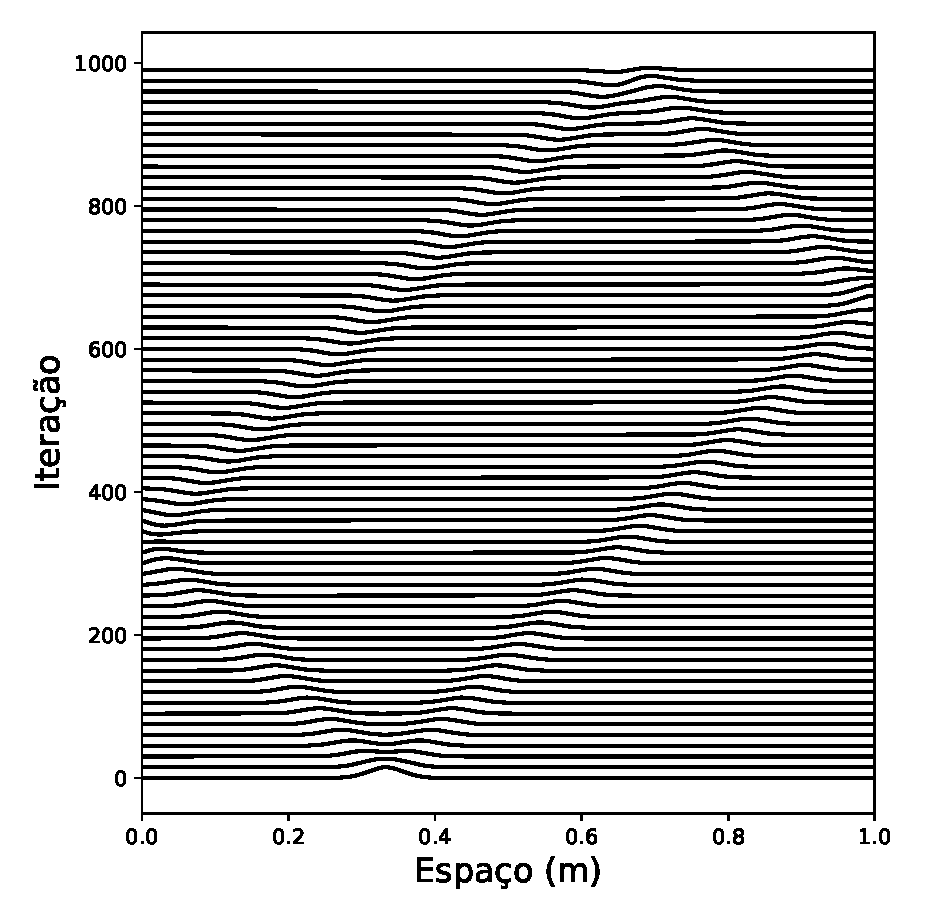
\includegraphics[width=0.45\textwidth]{evolucao-item-c}
    \label{fig:evolucao-item-c}
\end{figure}




Observa-se que os modos multíplos de \( 3 \) e \( 4 \) não compõem o espectro de potências.


\begin{figure}[h!] 
    \centering
    \caption{}
    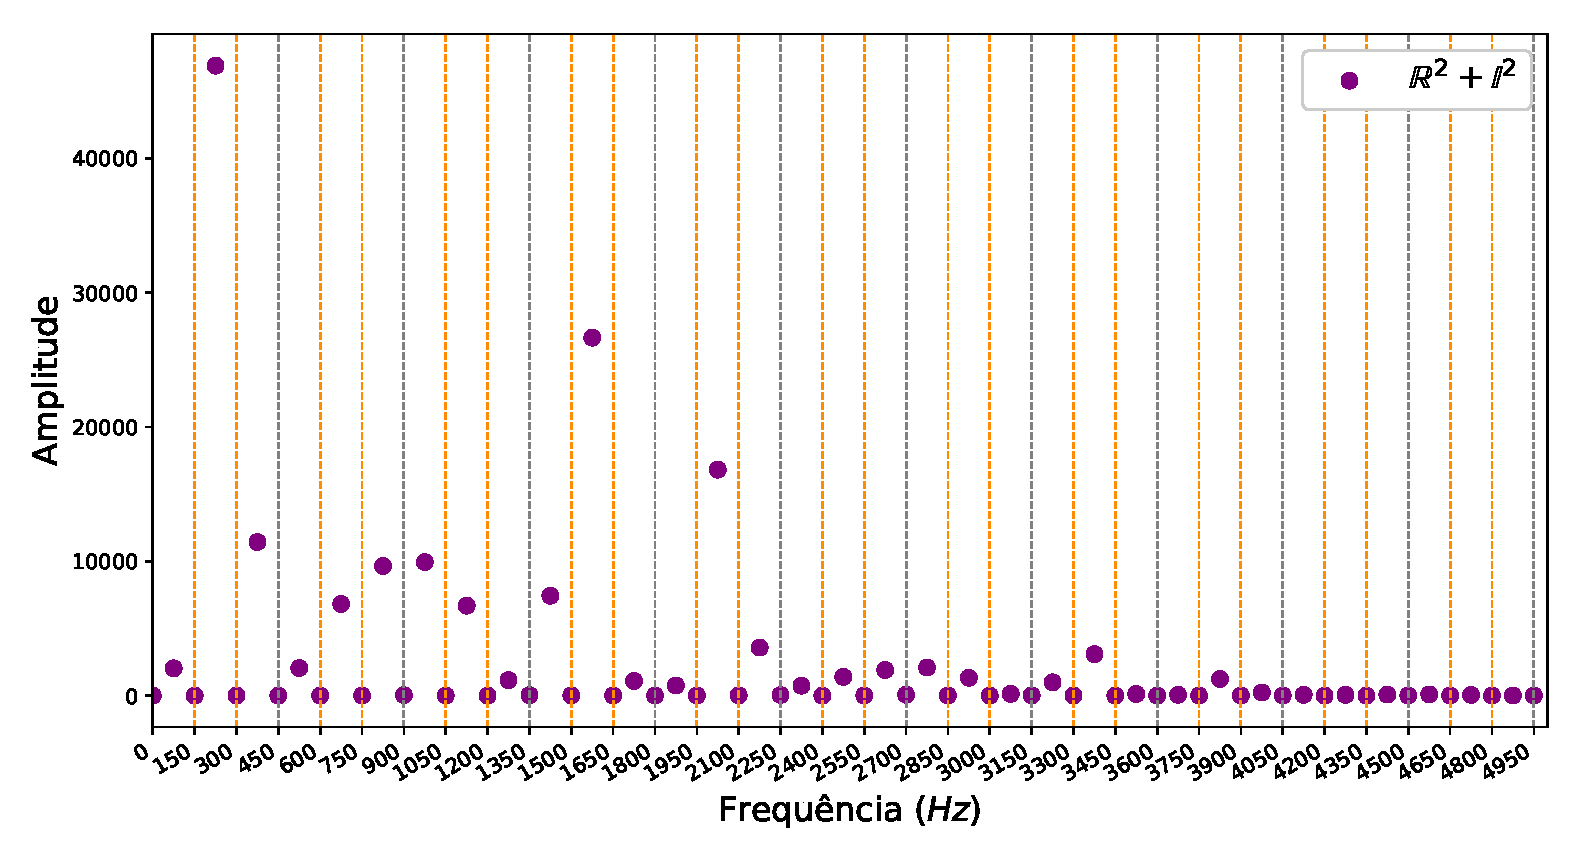
\includegraphics[width=0.65\textwidth]{dft-item-c}
    \label{fig:dft-item-c}
\end{figure}

As condições iniciais impostas nessa simulação são tais que os senos se anulam para frequências
fundamentais multíplas de \( 3 \). Isso também contribui para a amplitude do espectro observada para
as compomentes de termos pares.


\clearpage
\subsection{Simulação para \( x_0 = L/20 \) }

\begin{figure}[h!] 
    \centering
    \caption{}
    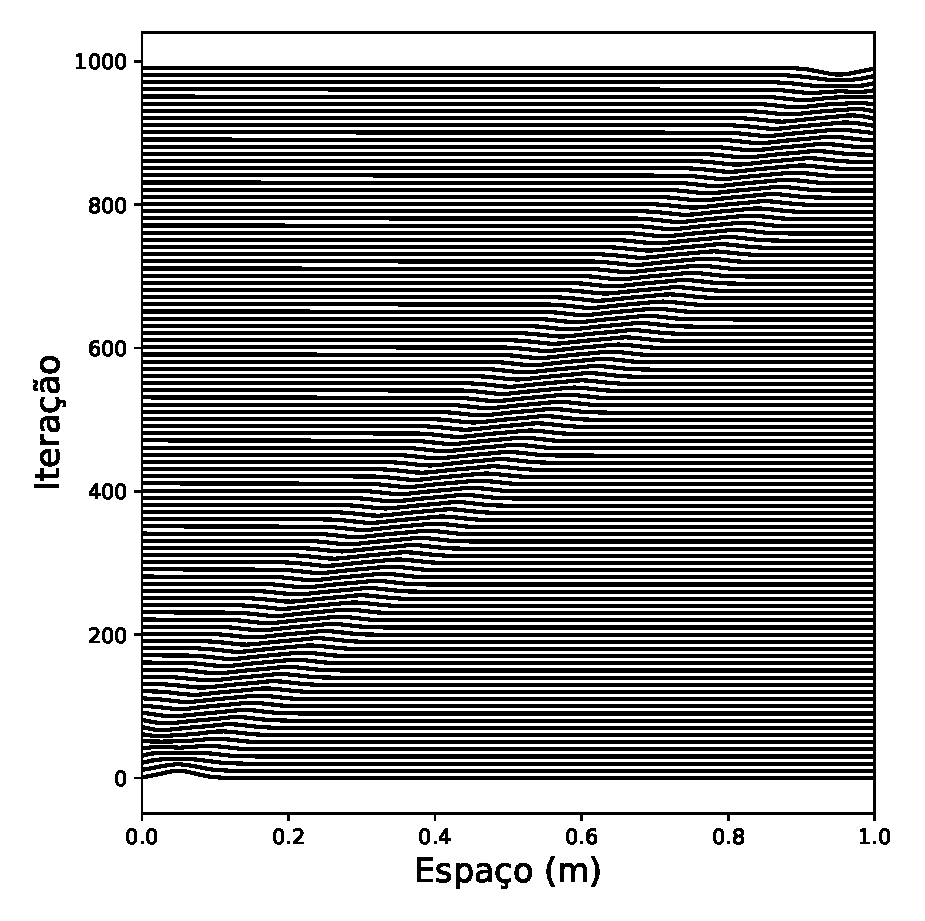
\includegraphics[width=0.45\textwidth]{evolucao-item-d}
    \label{fig:evolucao-item-d}
\end{figure}



Nessa condição as componentes espectrais tem aparência de gaussianas e não ficam tão
localizadas em pontos de frequências baixas como os resultados anteriores. Isso pode ser visto
pela diferença entre as componentes de frequência \( 300  \) (Hz) e \( 900 \) (Hz). Há um
salto muito grande entre \( 2 f_1 \) e \( 6 f_1  \).


\begin{figure}[h!] 
    \centering
    \caption{}
    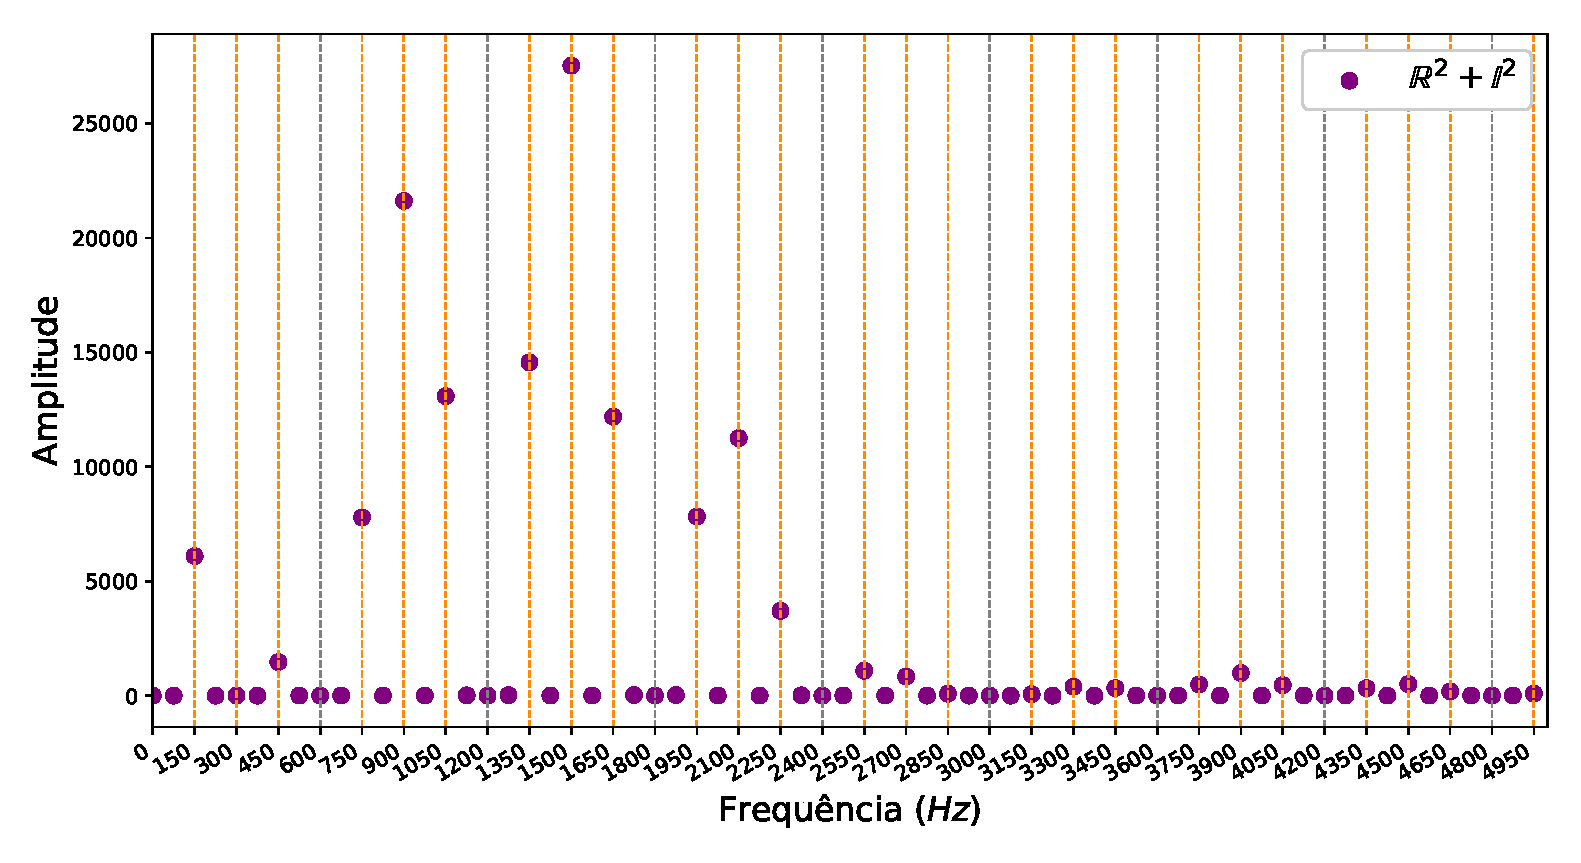
\includegraphics[width=0.65\textwidth]{dft-item-d}
    \label{fig:dft-item-d}
\end{figure}

Novamente os modos faltantes são os de mutíplos de \( 4n \).



\clearpage
\subsection{Simulação para \( x_0 = L/2 \) (Borda solta)}
Para a implementação dessa simulação foi mudado apenas a rotina chamada no programa principal e
executado.




Nota-se que na última iteração na figura (\ref{fig:evolucao-item-e}) podemos ver a forma da onda se propagando.
\begin{figure}[h!] 
    \centering
    \caption{}
    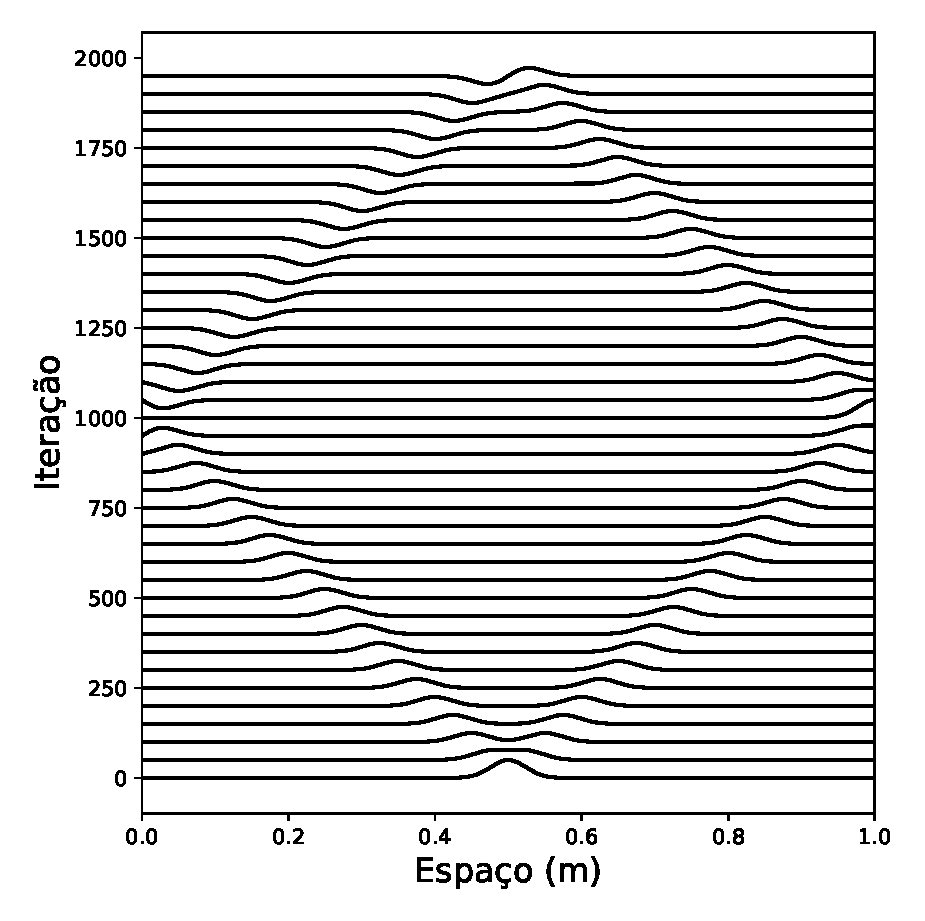
\includegraphics[width=0.45\textwidth]{evolucao-item-e}
    \label{fig:evolucao-item-e}
\end{figure}


Da figura (\ref{fig:dft-item-e}) podemos notar que as frequências fundamentais passam a
ser \( f_n  = \left( 75 + 150n \right)\)  (Hz), ou seja, há uma fase adicionada à componente
do seno, isso satisfaz a condição de ser máximo em \( x = L \).


\begin{figure}[h!] 
    \centering
    \caption{}
    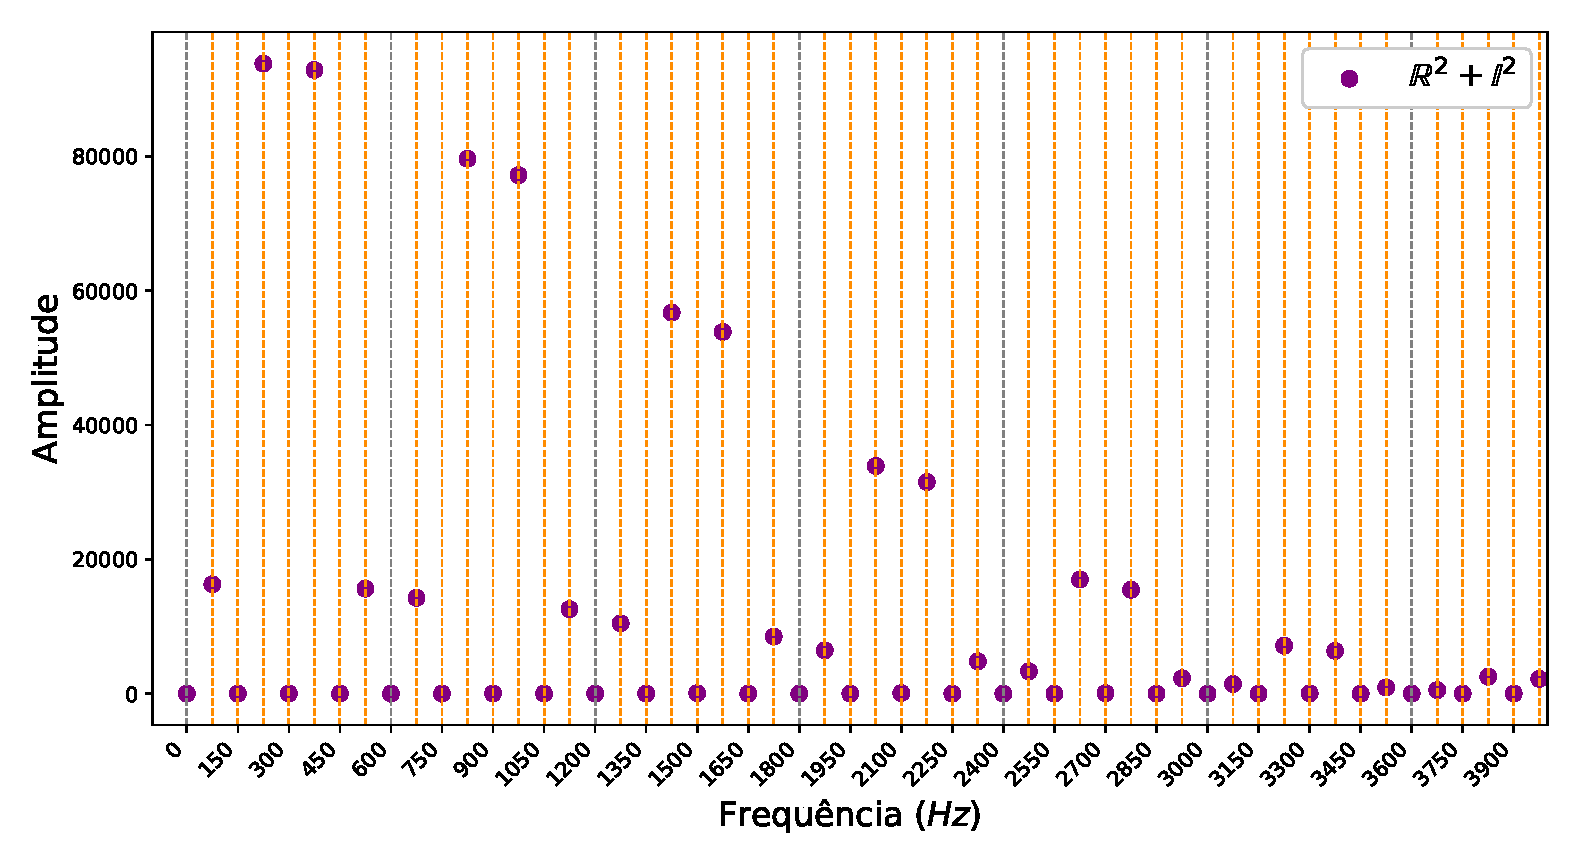
\includegraphics[width=0.65\textwidth]{dft-item-e}
    \label{fig:dft-item-e}
\end{figure}
\end{document}
%%% Local Variables:
%%% mode: latex
%%% TeX-master: "main.tex"
%%% End:
